\newpage
\section{Generowanie ruchów}
\label{sec:generowanie-ruchow}

Generowanie możliwych ruchów w danej pozycji jest jednym z podstawowych, ale~też~kluczowych elementów każdego silnika szachowego.
Jego efektywna implementacja ma znaczący wpływ na wydajność całego systemu.
Opisane w poprzednim podroździale struktury danych reprezentacji szachownicy w dużym stopniu zdeterminowały techniki, które zostały wykorzystane w generatorze.

Podstawowym rozróżnieniem stosowanych rozwiązań jest podział na generowanie ruchów pseudolegalnych oraz ruchów legalnych.
Ruch pseudolegalny to taki, który nie narusza zasad ruchów poszczególnych bierek, natomiast istnieje możliwość, że po jego wykonaniu własny król znajdzie się w szachu.
Takie rozwiązanie jest możliwe do zaimplementowania, z~uwagi na pozostawienie odpowiedzialności za sprawdzenie legalności ruchu funkcji ten ruch wykonującej.
Główną zaletą tego rozwiązania jest znacznie łatwiejsza implementacja.

\subsection{Operacje na mapach bitowych}
\label{subsec:operacje-na-mapach-bitowych}

\subsubsection{Generowanie ruchów piona}

Pion ma do dyspozycji parę możliwych ruchów, które należało zaimplementować: ruch o~jedno pole do przodu, ruch o dwa pola do przodu, bicie w lewo, bicie w prawo oraz ruch en-passant.
Każdy z graczy zaczyna rozgrywkę z ośmioma pionami, a w większości partii ich ilość pozostaje znaczna aż do zakończenia rozgrywki.
Czasochłonna wydawała się więc iteracja po~wszystkich bierkach tego typu i indywidualne generowanie ruchów dla każdego z osobna.
Z tego względu wykorzystano operacje bitowe i przesunięcia na masce bitowej.

Poniżej przykład generowania ruchów dla białych pionków.
\begin{align*}
    moves & = empty && \text{pole końcowe musi być puste} \\
    moves & = moves \wedge (P_w\ll16) && \text{pionek musi być dwa wiersze niżej}\\
    moves & = moves \wedge (empty\ll8) && \text{wiersz niżej musi być pusty}\\
    moves & = moves \wedge rank4 && \text{pole końcowe musi być w czwartym wierszu}
\end{align*}

\begin{figure}[ht]
    \centering
    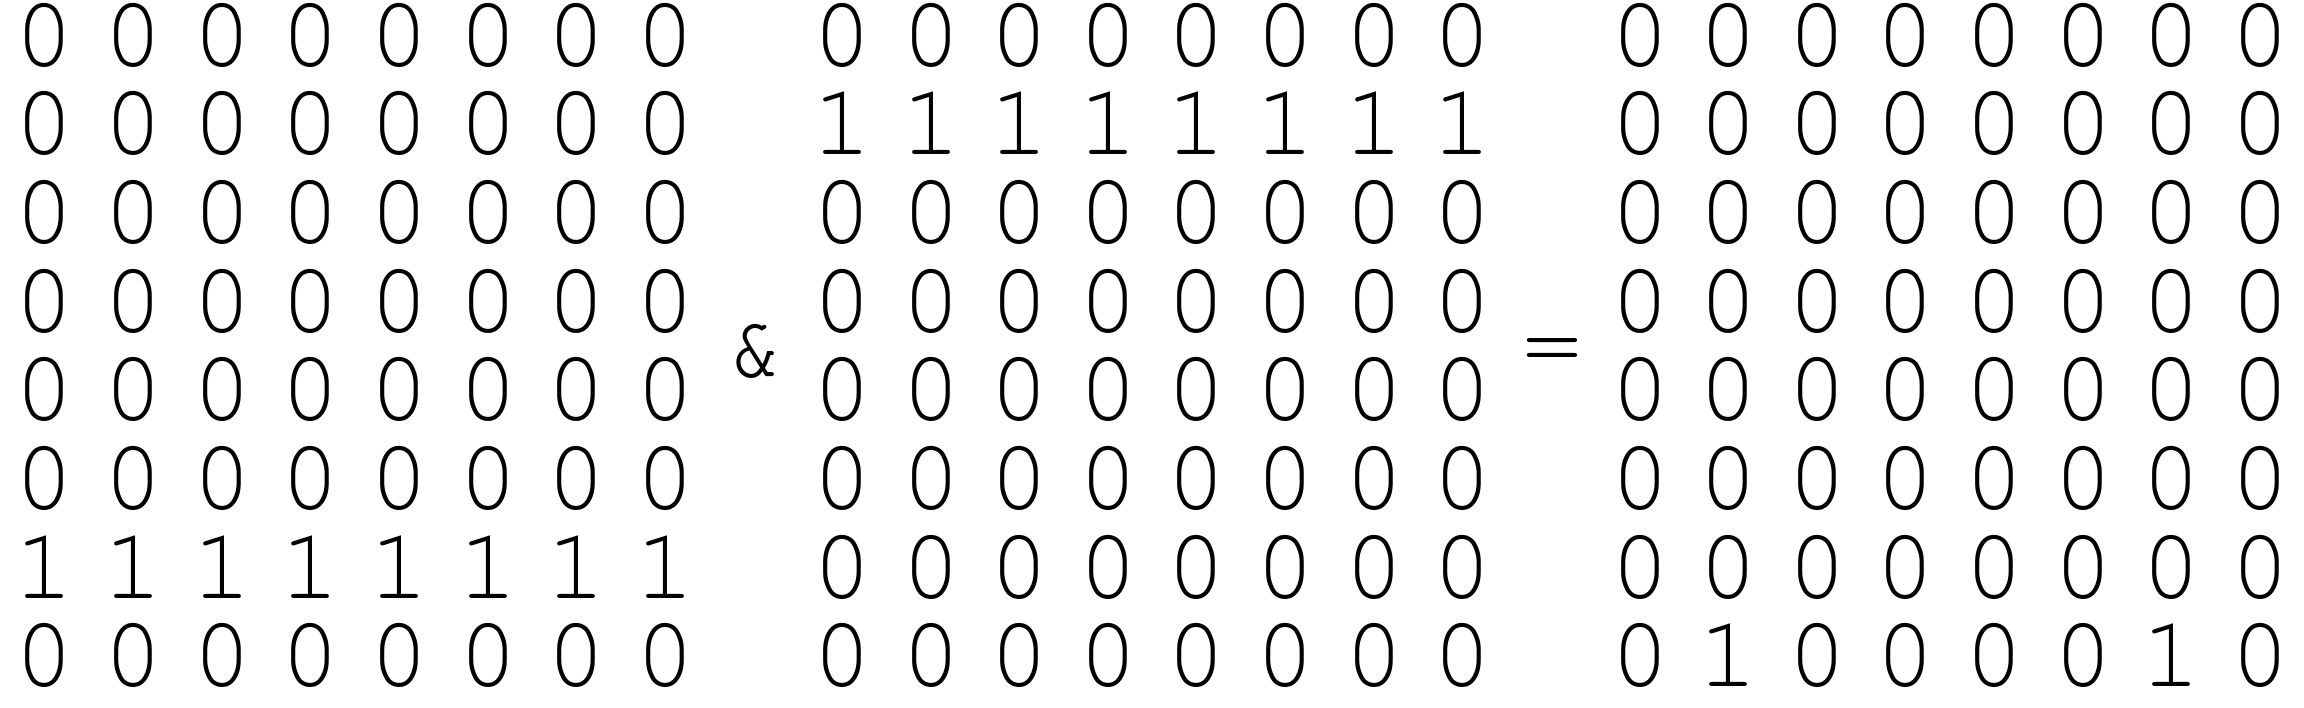
\includegraphics[width=0.85\linewidth]{rozdzialy/rozdzial01/3_generowanie-ruchow/rysunki/bitboards-arithmetic}
    \caption{Kodowanie ruchu szachowego}
    \label{fig:bitboards-arithmetic}
\end{figure}


\subsubsection{Generowanie ruchów hetmana, wieży i gońca}

Ruchy hetmana są połączeniem ruchów wieży oraz gońca, z tego względu można je generować w ten sam sposób.
Techniki te operują na bardzo podobnych zasadach, co generowanie ruchów piona, z tą różnicą, że figury mogą poruszać się o dowolną liczbę pól w danym kierunku, aż do momentu napotkania innej bierki na swojej drodze.
Aby uniknąć skomplikowanych obliczeń, należało zaimplementować funkcję, która w literaturze znana jest pod nazwą (ang.~\emph{Hyperbola Quintessence}).

$lineAttacks =   (o-2r) \string^ reverse( o'-2r')$

\subsubsection{Generowanie ruchów króla i skoczka}


\subsection{Hyperbola Quintessence}
\label{subsec:hyperbola-quintessence}

Generowanie ruchów hetmana, wieży i gońca odbywa się w sposób odmienny.
Wynika to~z~faktu, że figury te poruszają się~o~dowolną liczbę pól w danym kierunku, aż do momentu napotkania innej bierki na swojej drodze.
W przypadku bierki przeciwnika możliwe jest bicie, w przypadku bierki własnej, należy zatrzymać się pole wcześniej.
Choć są to trzy różne figury, to mają do dyspozycji dwa możliwe ruchy, ruch w linii prostej, jak wieża, oraz ruch po przekątnej, jak~goniec.
Ruchy hetmana są natomiast sumą dwóch powyższych generatorów.

Większość silników szachowych korzystających z masek bitowych implementuje funkcję, która w literaturze zwana jest jako ang. \emph{Hyperbola Quintessence}.
Pozwala ona na wygenerowanie dostępnych ruchów w jednej prostej oraz na uniknięcie zawiłej logiki iteracyjnej.
\begin{align*}
    o = \text{11010101} && o' = \text{10101011} && \text{pola zajęte przez bierki} \\
    r = \text{00010000} && r' = \text{00001000} && \text{pole figury dla której generujemy ruchy} \\
    o-r = \text{11000101} && o'-r' = \text{10100011} && \text{pola zajęte minus pole figury} \\
    \alpha = o-2r = \text{10110101} && \beta = o'-2r' = \text{10011011} && \text{pola zajęte dwukrotnie minus pole figury} \\
    (\alpha \oplus \beta') \wedge \neg \gamma && \text{01101100} && \text{maska legalnych ruchów}
\end{align*}
\begin{multicols}{2}
    \begin{itemize}[label={}]
        \item \(\oplus\) — alternatywa wykluczająca
        \item \(\wedge\) — koniunkcja
        \item \(x'\) — odwrócenie bitów
        \item \(\gamma\) — maska pól zajętych przez własne bierki
    \end{itemize}
\end{multicols}





\subsection{Ruchy specjalne}
\label{subsec:ruchy-specjalne}

Pozostałymi ruchami do zaimplementowania było bicie w przelocie oraz cztery roszady.
Z uwagi na znikomą liczbę takich posunięć w danej pozycji oraz na złożoną logikę tych ruchów, zostały one wygenerowane explicite z zasad gry.

Oba typy ruchów wymagały dodatkowej weryfikacji z danymi dostępnymi w reprezentacji stanu gry.
Pierwszy z nich – en-passant – został wygenerowany przez nałożenie na siebie maski pola bicia w przelocie oraz maski pionów, odpowiednio przesuniętych o $\pm 7$ oraz $\pm 9$ kratek.

Aby uzyskać prawo roszady, należy spełnić następujące warunki:
\begin{enumerate}
    \item Ani król, ani wieża biorąca udział w roszadzie nie mogły wykonać wcześniej ruchu.
    \item Pola między królem a wieżą muszą być puste.
    \item Król nie może znajdować się w szachu.
    \item Król nie może przechodzić bądź kończyć ruch na polach atakowanych przez bierki przeciwnika.
\end{enumerate}




\subsection{Generowanie ruchów legalnych}
\label{subsec:generowanie-ruchow-legalnych}

\subsubsection{Technika usuwania ruchów pseudo-legalnych}

Po zaimplementowaniu logiki opisanej powyżej, silnik był zdolny do generowania posunięć pseudolegalnych.
Natomiast ruch, po którym własny król znajduje się w szachu, nie tylko jest ruchem nieoptymalnym, ale również z punktu widzenia reguł FIDE nielegalnym.

W literaturze można znaleźć kilka podejść do problemu odfiltrowywania ruchów pseudolegalnych.
Niektóre z nich korzystają z dodatkowych masek bitowych, reprezentujących pola atakowane przez bierki danej strony.
W niniejszej implementacji zastosowano jednak rozwiązanie, w subiektywnym odczuciu autora, łatwiejsze.

Po wykonaniu konkretnego ruchu, w miejscu, gdzie znajduje się król, stawiane są kolejne figury oraz generowane są dostępne bicia.
Jeśli wśród bić znajduje się bierka przeciwnika, tego samego typu, co aktualnie podstawiona, oznacza to, że król znajduje się w szachu, a więc posunięcie nie należy do kategorii ruchów legalnych.

\subsubsection{Test wydajności}

Generatory ruchów szachowych posiadają skomplikowaną logikę.
Z tego względu bardzo łatwo o popełnienie błędu w implementacji.
Dopuszczenie choćby jednego błędu, skutkować będzie jego propagacją na większych głębokościach, a w skrajnych przypadkach doprowadzi do~zakończenia programu.

Ocena poprawności metodą przeprowadzania rozgrywek z silnikiem szachowym jest~rozwiązaniem czasochłonnym.
Odwiedzenie dużej ilości węzłów drzewa gry, w~celu~sprawdzenia poprawności wykonywania ruchów, jest praktycznie niemożliwe.
Błędy w~ten~sposób powstałe są trudne do zlokalizowania.

Z tego względu zastosowano Test Wydajności (ang.~\emph{Performance Testing}, w~skrócie Perft~Test).
Choć nazwa mogłaby wskazywać na testowanie prędkości generowanych ruchów, test ten można przeprowadzić także w celu kontroli poprawności.
Metoda ta~opiera się~na~wykorzystaniu algorytmu DFS dla ograniczonej głębokości na drzewie gry, przy jednoczesnym zliczaniu odwiedzonych węzłów.
Tak otrzymane wyniki można porównać z konsensusem osiągniętym przez twórców silników szachowych.
Jako punkt odniesienia autor przyjął wyniki generowane przez silnik Stockfish.
Przeprowadzenie testów z różnych pozycji startowych oraz dla~różnych głębokości pozwoliło na potwierdzenie poprawności implementowanego generatora, z~prawdopodobieństwem graniczącym z pewnością.
Przykładowe wyniki zaprezentowano w dodatku \ref{ch:wyniki-perft}.

